\documentclass[prb,twocolumn,superscriptaddress,amsmath,amssymb,floatfix]{revtex4-2}
\usepackage{graphicx}
\usepackage{bm}
\usepackage[colorlinks=true,linkcolor=blue,citecolor=blue,urlcolor=blue]{hyperref}
\newcommand{\todo}[1]{\textcolor{red}{[#1]}}
\newcommand{\Jb}{\bar J}

\begin{document}

\title{Honeycomb, dice and triangle: the $S_3$ phase diagram of the three-coupling\\ spin-1/2 triangular-lattice Heisenberg antiferromagnet}

\author{Changyeon Won}
\affiliation{Department of Physics, Kyung Hee University, Seoul, Republic of Korea}

\date{Draft, \today}

\begin{abstract}
The Heisenberg antiferromagnet on the $\sqrt3\times\sqrt3$-distorted triangular lattice has three nearest-neighbor couplings $J_{AB},J_{BC},J_{CA}$. Their space is a triangle acted on by $S_3$, whose vertices, edge midpoints and center are the honeycomb, dice and triangular lattices. We show that the classical ground state is non-collinear exactly when $1/J_{AB},1/J_{BC},1/J_{CA}$ obey the triangle inequality and is a Lieb--Mattis ferrimagnet with $M=M_s/3$ otherwise. The saturation field $9S\bar J(1+\varepsilon)$ depends only on the size $\varepsilon$ of the anisotropy, while the $1/3$ plateau is centered at $3SJ_{\min}$, with the down sublattice opposite the weakest bond. Exact diagonalization of 18 and 27 spins $S=1/2$ confirms these structures and shows that partial disorder survives only in a wedge of width $\propto J'^2/J$ around the honeycomb-direction mirrors. On these mirrors the classical plateau width vanishes. Fluctuations of the polarized hub spins select the collinear state of the honeycomb rim by order by disorder, which produces a plateau of width $\propto\sqrt S$ bounded by first-order spin flops. A quantum-rotor description with no fitted parameter accounts for the plateau widths of finite clusters and for the growth of the rim anisotropy with cluster size. A resonance efficiency measures how far the three honeycomb N\'eel orders can be satisfied at once.
\end{abstract}

\maketitle

%=====================================================================
\section{Introduction}
Lattices built from two inequivalent sites interpolate between the classic frustrated and unfrustrated antiferromagnets. The $\sqrt3\times\sqrt3$-distorted triangular lattice is the simplest case: its three sublattices $A,B,C$ are connected by three couplings $J_{AB},J_{BC},J_{CA}$. Switching on one coupling gives the honeycomb lattice with its N\'eel order; two give the dice lattice, a Lieb--Mattis ferrimagnet~\cite{LiebMattis1962}; all three equal give the triangular lattice, with $120^\circ$ order and a $1/3$ magnetization plateau stabilized by quantum fluctuations~\cite{ChubukovGolosov1991}. Rare-earth indium oxides realize the intermediate case as centered-honeycomb layers; GdInO$_3$, whose Gd$^{3+}$ moments are close to isotropic, shows an up-up-down $1/3$ plateau~\cite{Yuan2023}.

Earlier work followed single lines through this space. On the honeycomb side, weak coupling to the central (hub) spins leaves them disordered while the honeycomb orders, the partially disordered state~\cite{Gonzalez2019,SeifertVojta2019}; a related state occurs on the stuffed square lattice~\cite{Blesio2023}. Between the triangular and dice points numerical work found ferrimagnetism and an intermediate phase~\cite{NakanoSakai2017,NakanoSakai2018,Shimada2018,Shimada2018b}, and the classical phase diagram of the stuffed honeycomb lattice is known~\cite{Sahoo2018}. These lines are pieces of one parameter space, and it has been open how the honeycomb, dice and triangular limits connect across it, in zero field and in a magnetic field.

Here we treat the full coupling space. Its structure follows from $S_3$ symmetry and a few closed formulas, each tested by exact diagonalization on 18 and 27 sites. The classical ground state is non-collinear exactly when the inverse couplings obey the triangle inequality (Sec.~\ref{sec:zero}). Partial disorder is confined to a wedge of width $\propto J'^2/J$ around the honeycomb-direction mirrors. Three honeycomb N\'eel orders compete for the same spins, and a resonance efficiency measures how far they can be satisfied together (Sec.~\ref{sec:resonance}). In a field the saturation field depends only on the size of the anisotropy, and the $1/3$ plateau is fixed by the weakest bond (Sec.~\ref{sec:field}). On the honeycomb mirror the classical plateau width vanishes; there the plateau arises from order by disorder driven by the hub spins and ends in spin flops, with a width of order $\sqrt S$ instead of the $S^0$ of the triangular lattice.

%=====================================================================
\section{Model and $S_3$ structure}
\label{sec:model}

We divide the triangular lattice into three $\sqrt3\times\sqrt3$ sublattices $A$, $B$, $C$ and assign one exchange constant to each pair of sublattices,
\begin{equation}
H=\sum_{\langle ij\rangle}J_{s_is_j}\,\mathbf S_i\cdot\mathbf S_j-h\sum_i S_i^z ,\qquad J_{AB},J_{BC},J_{CA}\ge0 .
\label{eq:H}
\end{equation}
Every site has three bonds of each type that touches its sublattice [Fig.~\ref{fig:model}(a)]. Switching on a single coupling gives a honeycomb lattice plus decoupled spins on the third sublattice; two couplings give the dice lattice, whose shared sublattice is the six-coordinated hub; three equal couplings give the triangular lattice. The Hamiltonian is linear in the couplings,
\begin{equation}
H=J_{AB}H_{AB}+J_{BC}H_{BC}+J_{CA}H_{CA},
\label{eq:linear}
\end{equation}
where $H_{ss'}$ is the Heisenberg Hamiltonian of the honeycomb lattice formed by sublattices $s$ and $s'$.

\paragraph{Symmetry.}
The primitive translation $t$ of the triangular lattice permutes the sublattices cyclically ($A\to B\to C$), and a site-centred inversion exchanges two of them. These lattice operations generate $S_3\cong D_3$ acting on $w=(J_{AB},J_{BC},J_{CA})$. The coupling vector decomposes as $A_1\oplus E$: the mean $\Jb$ and a two-component anisotropy $(\varepsilon,\varphi)$,
\begin{equation}
J_k=\Jb\left[1+2\varepsilon\cos\!\left(\varphi-\tfrac{2\pi k}{3}\right)\right],\qquad k=0\,(AB),\,1\,(BC),\,2\,(CA).
\label{eq:Erep}
\end{equation}
At fixed $\Jb$ the physical region $J_k\ge0$ is a triangle in the $(\varepsilon\cos\varphi,\varepsilon\sin\varphi)$ plane [Fig.~\ref{fig:model}(b)]. Its vertices ($\varepsilon=1$, $\varphi=0,2\pi/3,4\pi/3$) are the three honeycomb lattices, the midpoints of its edges ($\varepsilon=1/2$, $\varphi=\pi/3,\pi,5\pi/3$) are the three dice lattices, and its centre is the triangular lattice. The six mirror lines divide it into equivalent fundamental domains; we use $0\le\varphi\le\pi/3$, in which $J_{CA}$ is the weakest coupling. The three sides of this domain are
(i) the honeycomb-direction mirror $\varphi=0$, $J_{AB}>J_{BC}=J_{CA}$, the line $r=J'/J=(1-\varepsilon)/(1+2\varepsilon)<1$ studied in Refs.~\cite{Gonzalez2019,SeifertVojta2019};
(ii) the dice-direction mirror $\varphi=\pi/3$, $J_{AB}=J_{BC}>J_{CA}$, equivalent to $r=(1+\varepsilon)/(1-2\varepsilon)>1$~\cite{NakanoSakai2017};
(iii) the edge $J_{CA}=0$ joining a honeycomb lattice to a dice lattice.

The invariants of the $E$ representation are $\varepsilon^2$ and $\varepsilon^3\cos3\varphi$. Because no linear invariant exists, the triangular point is a stationary point of every symmetric quantity, and the cubic invariant is the lowest-order term that distinguishes the honeycomb direction ($\cos3\varphi=+1$) from the dice direction ($\cos3\varphi=-1$). This is why physics on the two sides of the triangular point along the old $r$ line is asymmetric.

\begin{figure*}[tbp]
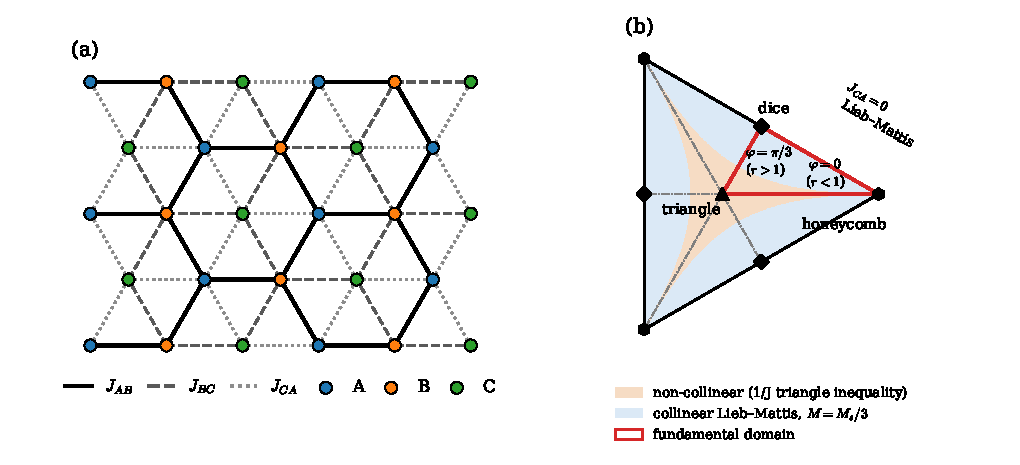
\includegraphics[width=0.9\textwidth]{figures/fig1_model.pdf}
\caption{Honeycomb, dice and triangular lattices are the vertices, edge midpoints and centre of one coupling triangle. (a) Three-coupling triangular lattice: sublattices $A,B,C$ and the three bond types. (b) Coupling triangle in the plane of the $E$ anisotropy $(\varepsilon\cos\varphi,\varepsilon\sin\varphi)$ at fixed $\Jb$, with mirror lines (dash-dotted) and the fundamental domain (red). Shading: classical ground state, non-collinear where $1/J_{AB},1/J_{BC},1/J_{CA}$ satisfy the triangle inequality [Eq.~\eqref{eq:triangle}], collinear Lieb--Mattis ferrimagnet otherwise.}
\label{fig:model}
\end{figure*}

%=====================================================================
\section{Zero field}
\label{sec:zero}

\subsection{Classical ground state: a triangle inequality for $1/J$}
For three-sublattice states of unit vectors $\mathbf a,\mathbf b,\mathbf c$ the energy per cell is $3S^2(J_{AB}\,\mathbf a\!\cdot\!\mathbf b+J_{BC}\,\mathbf b\!\cdot\!\mathbf c+J_{CA}\,\mathbf c\!\cdot\!\mathbf a)$. With
$\alpha=\sqrt{J_{AB}J_{CA}/J_{BC}}$, $\beta=\sqrt{J_{AB}J_{BC}/J_{CA}}$, $\gamma=\sqrt{J_{BC}J_{CA}/J_{AB}}$ it can be written as a square (Appendix~\ref{app:three}),
\begin{equation}
\frac{E_{\rm cl}}{3S^2N_c}=\tfrac12\left|\alpha\mathbf a+\beta\mathbf b+\gamma\mathbf c\right|^2-\tfrac12\left(\alpha^2+\beta^2+\gamma^2\right).
\label{eq:square}
\end{equation}
The minimum $-\tfrac12(\alpha^2+\beta^2+\gamma^2)$ is reached when the weighted vectors close a triangle, which is possible if and only if
\begin{equation}
\frac1{J_{AB}}\le\frac1{J_{BC}}+\frac1{J_{CA}}\quad\text{and cyclic},
\label{eq:triangle}
\end{equation}
since $(\alpha,\beta,\gamma)\propto(1/J_{BC},1/J_{CA},1/J_{AB})$. The angles follow from the closed triangle, $\mathbf a\cdot\mathbf b=(\gamma^2-\alpha^2-\beta^2)/2\alpha\beta$ and cyclic, and the classical magnetization is $M/M_s=|\mathbf a+\mathbf b+\mathbf c|/3$. Outside the region~\eqref{eq:triangle} the minimum is collinear: the two ends of the weakest bond are parallel and the third sublattice is antiparallel, giving $M=M_s/3$. On the dice mirror this boundary is $r=2$; near a honeycomb vertex it is the wedge $|J_{BC}-J_{CA}|\le J_{BC}J_{CA}/J_{AB}$ around the honeycomb mirror. Along the honeycomb mirror the state is non-collinear all the way to the vertex, with $M/M_s=(1-r)/3$.

\subsection{The Lieb--Mattis edge}
On the edge $J_{CA}=0$ the lattice is bipartite, $\{B\}$ versus $\{A,C\}$, and the Lieb--Mattis theorem~\cite{LiebMattis1962} fixes the ground-state spin to $S_{\rm tot}=|N_A+N_C-N_B|/2=N/6$ for all $J_{AB},J_{BC}>0$. This is an exact statement for any spin $S$; on 18-spin clusters we find $S_{\rm tot}=3$ for every $J_{BC}/J_{AB}$ tested.

\subsection{Quantum ground state on finite clusters}
\begin{figure*}[tbp]
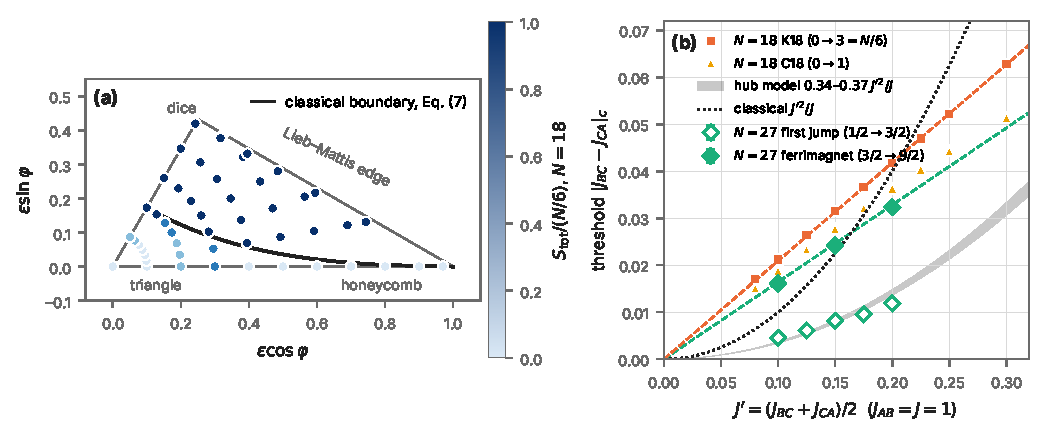
\includegraphics[width=\textwidth]{figures/fig2_zero_field.pdf}
\caption{Zero field. (a) Ground-state spin of the 18-site cluster (K18) over the fundamental domain, in the plane $(\varepsilon\cos\varphi,\varepsilon\sin\varphi)$. The black line is the classical boundary~\eqref{eq:triangle}; outside it the ground state is the Lieb--Mattis ferrimagnet, $S_{\rm tot}=N/6$. (b) Half-width of the partially disordered wedge around the honeycomb mirror, $J_{AB}=1$, $J_{BC,CA}=J'\pm\delta/2$: the first jump of $S_{\rm tot}$ on two 18-site clusters and on 27 sites (bisection brackets), compared with the finite-size scaling $0.14J'$ projected from 18 sites, the hub-model estimate~\eqref{eq:wedge} and the classical wedge.}
\label{fig:zero}
\end{figure*}
Exact diagonalization of two 18-site clusters on 55 points of the fundamental domain shows that the ground state reaches $S_{\rm tot}=N/6$ at the classical boundary within the grid resolution $\Delta\varepsilon=0.1$ in every direction $10^\circ\le\varphi\le60^\circ$. Near the triangular point and along the honeycomb mirror the spin is smaller, and on the honeycomb mirror at small $r$ it is zero, the partially disordered state~\cite{Gonzalez2019}.

\subsection{Partial disorder is confined to a wedge}
Away from the honeycomb mirror the N\'eel order of the rim exerts a uniform static field $3m_N(J_{BC}-J_{CA})$ on every hub spin, because each hub has three $A$ and three $B$ neighbours. On the mirror this field vanishes by symmetry. The hubs therefore stay disordered only while the field is smaller than the saturation field of their effective model, generated at second order in $J'$ by the rim magnons~\cite{SeifertVojta2019}. We recomputed the leading transverse couplings from the linear-spin-wave N\'eel state (Appendix~\ref{app:hub}); they reproduce Table~I of Ref.~\cite{SeifertVojta2019} and satisfy an exact sum rule. With the $S=1/2$ couplings of Ref.~\cite{SeifertVojta2019}, in which the $1/S$ correction cancels 97\% of the classical transverse coupling, the hub saturation field is $0.27\,J'^2/J$ and the wedge is
\begin{equation}
|J_{BC}-J_{CA}|\lesssim(0.34\text{--}0.37)\,\frac{J'^2}{J},\qquad J'=\tfrac12(J_{BC}+J_{CA}),\ J=J_{AB}.
\label{eq:wedge}
\end{equation}
This is narrower than the classical non-collinear wedge $J'^2/J$. On 18 sites the jump of $S_{\rm tot}$ occurs at $|J_{BC}-J_{CA}|=0.21J'$ (and $0.19J'$ on the second cluster), linear in $J'$, which on its own would mean a finite-size effect; scaling with the number of hubs predicts $0.14J'$ on 27 sites. The 27-site cluster gives instead $|J_{BC}-J_{CA}|_c\in(0.0075,0.0088]$ at $J'=0.15$ and $(0.0113,0.0125]$ at $J'=0.2$ [Fig.~\ref{fig:zero}(b)], i.e.\ $|J_{BC}-J_{CA}|_c/J'^2=0.28$--$0.39$, nearly independent of $J'$ and of the magnitude given by Eq.~\eqref{eq:wedge}. Between 18 and 27 sites the threshold falls by a factor 0.24--0.34, much faster than the $2/3$ of finite-size scaling. The wedge therefore has a bulk width $\propto J'^2/J$, set by the effective hub couplings. The ED threshold marks the onset of hub magnetization ($S_{\rm tot}=1/2\to3/2$), while Eq.~\eqref{eq:wedge} is a saturation criterion, so only the $J'^2$ scaling, not the prefactor, should be read as confirmed.

%=====================================================================
\section{Resonance of honeycombs}
\label{sec:resonance}
Because $H$ is linear in $w$ [Eq.~\eqref{eq:linear}], its ground-state energy $E(w)$ is concave and homogeneous of degree one, so $E(w)\ge\sum_kJ_kE_{\rm hex}$, with equality only if the three honeycomb Hamiltonians share a ground state. We define the resonance efficiency
\begin{equation}
f(w)=\frac{E(w)}{\sum_kJ_kE_{\rm hex}}\in[0,1],
\label{eq:f}
\end{equation}
and the satisfaction of honeycomb $k$, $s_k=\langle H_k\rangle/E_{\rm hex}=\partial E/\partial J_k\,/E_{\rm hex}$ (Hellmann--Feynman). Classically, from Eq.~\eqref{eq:square},
\begin{equation}
f_{\rm cl}=
\begin{cases}
\dfrac{\alpha^2+\beta^2+\gamma^2}{2\sum_kJ_k} & \text{non-collinear},\\[2ex]
\dfrac{J_1+J_2-J_{\min}}{\sum_kJ_k} & \text{collinear}.
\end{cases}
\end{equation}
It is minimal, $f_{\rm cl}=1/2$, at the triangular point, where the three honeycomb N\'eel orders cannot be satisfied together because $A$--$B$--$C$ is an odd loop. On the dice lattice two honeycomb orders share the hub and are compatible, $f_{\rm cl}=1$.

On 18 sites $f=0.497$ at the triangular point, close to the classical value, and each honeycomb is half satisfied, $s_k=0.50$. In the Lieb--Mattis region the quantum $f$ falls well below the classical value (0.82 against 1 at the dice point). Linear spin-wave theory explains this: $f_{\rm LSWT}/f_{\rm cl}=(1+g_{\rm LM})/(1+g_{\rm hex})$, where $g$ is the zero-point gain relative to the classical energy, $g_{\rm hex}=0.42$ for the N\'eel honeycomb and $g_{\rm LM}=0.27$ for the dice ferrimagnet, whose ferromagnetic branch carries no zero-point motion. This gives $f_{\rm LSWT}=0.89$ at the dice point and reproduces the trend over the whole collinear region (Fig.~\ref{fig:resonance}). On 27 sites $f=0.857$ at the dice point and $0.853$ near the Lieb--Mattis edge at $\varphi=30^\circ$, moving from the 18-site values toward linear spin-wave theory.

\begin{figure}[tbp]
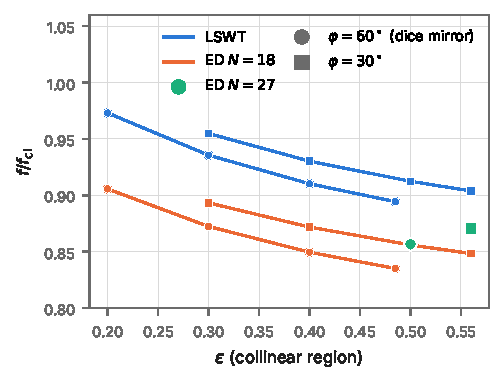
\includegraphics[width=\columnwidth]{figures/fig3_resonance.pdf}
\caption{Resonance efficiency in the collinear (Lieb--Mattis) region relative to its classical value, along $\varphi=30^\circ$ and the dice mirror $\varphi=60^\circ$: linear spin-wave theory, 18 sites (K18) and 27 sites.}
\label{fig:resonance}
\end{figure}

%=====================================================================
\section{Magnetic field}
\label{sec:field}

\subsection{Saturation field}
The one-magnon instability of the polarized state occurs at the cell $\Gamma$ point, where the magnon matrix is $-3S$ times the weighted Laplacian $L$ of the $A$--$B$--$C$ triangle (Appendix~\ref{app:hsat}). Hence
\begin{align}
h_{\rm sat}&=3S\,\lambda_{\max}(L)=3S\Big[\textstyle\sum_kJ_k+\sqrt{\sum_kJ_k^2-\sum_{i<j}J_iJ_j}\Big]\nonumber\\
&=9S\Jb(1+\varepsilon).
\label{eq:hsat}
\end{align}
Although $S_3$ allows a $\cos3\varphi$ dependence, $h_{\rm sat}$ depends only on the size of the anisotropy. Equation~\eqref{eq:hsat} agrees with exact diagonalization at 110 points on 18 sites and at five points on 27 sites to $10^{-14}$. That the minimum lies at $\Gamma$ is verified numerically on dense $k$ grids; we have not found a general proof.

\subsection{Which sublattice points down on the $1/3$ plateau}
The classical up-up-down states are labelled by the sublattice $k$ that points down. Their energies per cell,
\begin{equation}
E(k\!\downarrow)=3S^2\big(2J_{\rm opp}(k)-J_{AB}-J_{BC}-J_{CA}\big),
\label{eq:potts}
\end{equation}
where $J_{\rm opp}(k)$ is the bond not touching $k$, form a three-state Potts field linear in $(\varepsilon,\varphi)$. The down sublattice is the one opposite the weakest bond, i.e.\ the hub of the strongest dice lattice. The plateau state is unique for generic $\varphi$, twofold degenerate on the honeycomb mirror and threefold at the triangular point. Exact diagonalization confirms this pattern through the $C_2$ parity and the eigenvalues $1,\omega,\omega^2$ of $t$ in the $S^z=N/6$ sector.

\subsection{Plateau window}
Linear spin-wave stability of the selected state is lost at $\Gamma$ (Appendix~\ref{app:window}), which gives
\begin{equation}
h_\pm=3S\Big[J_{\min}\pm\sqrt{(J_1-J_{\min})(J_2-J_{\min})}\Big],
\label{eq:window}
\end{equation}
with $J_1,J_2$ the two stronger couplings. The plateau is centred at $3SJ_{\min}$ and its classical width,
\begin{equation}
W_{\rm cl}=12\sqrt3\,S\Jb\,\varepsilon\sqrt{\sin\varphi\,\sin(\varphi+\pi/3)},
\end{equation}
is linear in the Potts field and vanishes as $\sqrt\varphi$ on the honeycomb mirror. The condition $h_-=0$ coincides with the boundary~\eqref{eq:triangle}: the plateau reaches zero field exactly where the ground state becomes the Lieb--Mattis ferrimagnet. On the dice mirror Eq.~\eqref{eq:window} reduces to $3JS(2-r)\le h\le3J'S$. Exact diagonalization keeps both structures of Eq.~\eqref{eq:window} (Fig.~\ref{fig:edges}). The lower edge lies a constant $0.11\pm0.02$ below $h_-$ at every point, on 18 and on 27 sites. The upper edge is a single multiple of $h_+$, independent of the direction $\varphi$: $1.49$--$1.52$ on 18 sites and $1.42$--$1.45$ on 27 sites. The multiple decreases with size; its thermodynamic value is not determined by two cluster sizes.

\begin{figure*}[tbp]
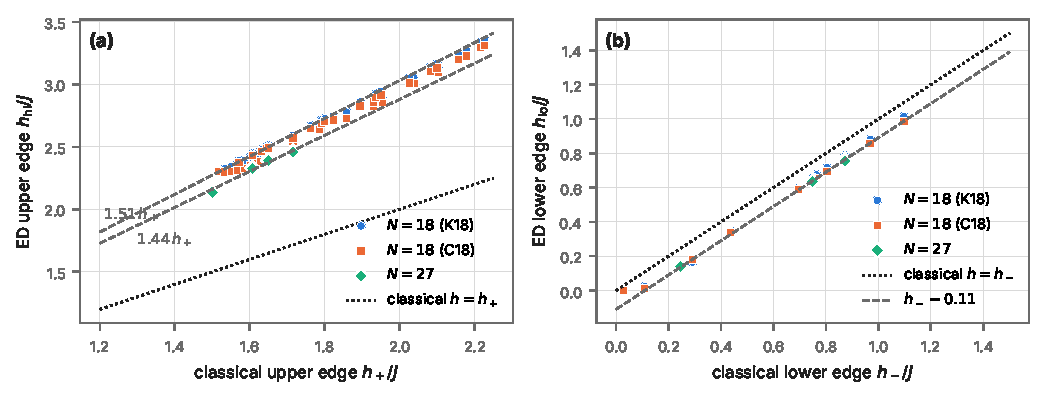
\includegraphics[width=\textwidth]{figures/fig4_plateau_edges.pdf}
\caption{Edges of the $1/3$ plateau off the honeycomb mirror ($\varphi\ge10^\circ$) against the classical window~\eqref{eq:window}. (a) Upper edge; dashed lines are $1.51\,h_+$ and $1.44\,h_+$. (b) Lower edge for $h_->0$; the dashed line is $h_--0.11$.}
\label{fig:edges}
\end{figure*}

\subsection{The honeycomb mirror}
On the honeycomb mirror, $J_{AB}=J$ and $J_{BC}=J_{CA}=rJ$ with $r<1$, the classical width vanishes and any plateau is a quantum effect. Expanding the classical energy in $\mathbf s=\mathbf a+\mathbf b$ at $h=3SrJ$ gives the quadratic form $\tfrac32S^2J\,[s_z^2+(1-r)|\mathbf s_\perp|^2]$ (Appendix~\ref{app:rotor}). For $r<1$ the classical ground states at this field are therefore the hubs fully polarized and the rim in a N\'eel state with an arbitrary direction $\mathbf n$: the exchange field of the hubs cancels the external field on the rim. Away from $h=3SrJ$ the rim flops perpendicular to the field with susceptibility $\chi=1/9$ per site, for every $r$ and $S$.

The zero-point energy of linear spin waves lifts this degeneracy. It is lowest for $\mathbf n\parallel\mathbf h$, the up-up-down state, by
\begin{equation}
K=E_{\rm zp}(\mathbf n\perp\mathbf h)-E_{\rm zp}(\mathbf n\parallel\mathbf h)=S\,k(r)\,J,
\label{eq:K}
\end{equation}
per site, with $k\approx0.09\,r^2$ for $r\lesssim0.2$ and $k=0.011,0.021,0.034$ at $r=0.4,0.6,0.8$. The angular dependence is $\sin^2\theta$ with a small negative $\sin^4\theta$ term, so the rim stays collinear until a first-order spin flop at $|h-3SrJ|=\sqrt{2K/\chi}$. The plateau width is
\begin{equation}
W=2\sqrt{2K/\chi}=6\sqrt{2S\,k(r)}\,J,
\label{eq:Wflop}
\end{equation}
of order $\sqrt S$. This is a different mechanism from the triangular point, where the order-by-disorder plateau has a width of order $S^0$~\cite{ChubukovGolosov1991}; Eq.~\eqref{eq:Wflop} holds for $(1-r)S\gg k$ and crosses over to the triangular case as $r\to1$.

On a cluster the rim N\'eel vector is a quantum rotor, $H_{\rm rot}=L^2/2I-D\,n_z^2$ with $I=\chi N$ and $D=NK$, and the plateau sector is $L_z=0$. Its width $W_N=2(E_{L_z=1}-E_{L_z=0})$ depends only on $x=\chi KN^2$: $W_NI=G(x)$ with $G(0)=2$, the tower of states, and $G\to2\sqrt{2x}$, Eq.~\eqref{eq:Wflop}, for $x\to\infty$ (Appendix~\ref{app:rotor}). With $\chi$ and $K$ from above and no fitted parameter, this reproduces the 27-site widths for $0.2\le r\le0.9$ to within 2--10\% [Fig.~\ref{fig:mirror}(a)]. All clusters available to exact diagonalization have $x\le1.7$, whereas the bulk regime $x\approx10$ needs $N\approx70$ ($r=0.8$) to $130$ ($r=0.4$). For small $x$, $W_N\simeq2/(\chi N)+0.27KN$ is not monotonic in $N$, so extrapolating two cluster sizes in $1/N$ is not meaningful here.

The selection itself is visible in the rim correlations. In the plateau sector the ratio of longitudinal to transverse nearest-neighbour correlations on the $A$--$B$ bonds exceeds its isotropic value $1/2$ by $\Delta$, while the neighbouring sectors are transverse [Fig.~\ref{fig:mirror}(b)]. For $x\ll1$ the rotor gives $\langle n_z^2\rangle-\tfrac13\propto x\propto N^2$, so $\Delta_{27}/\Delta_{18}=(27/18)^2=2.25$; a local anisotropy would give a ratio of 1. Exact diagonalization gives 2.0--3.0 at $r=0.4,0.6,0.8$ [Fig.~\ref{fig:mirror}(c)]. The orientation of the rim N\'eel vector, not a local effect, carries the selection, and it grows with system size at every $r$ we studied.

\begin{figure*}[tbp]
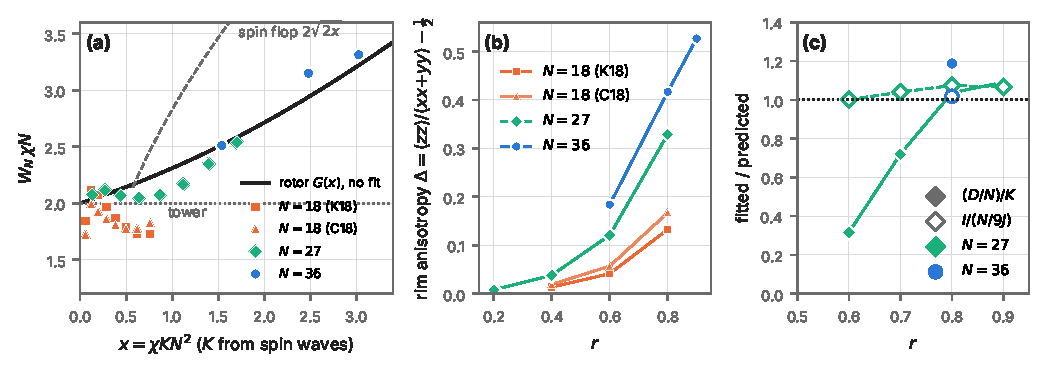
\includegraphics[width=\textwidth]{figures/fig5_mirror_plateau.pdf}
\caption{The $1/3$ plateau on the honeycomb mirror. (a) Width from exact diagonalization on 18 and 27 sites, the rotor theory for the same sizes (lines, no fitted parameter) and the bulk spin-flop width~\eqref{eq:Wflop} with $S=1/2$. (b) Rim anisotropy $\Delta$ in the plateau sector. (c) Size ratio $\Delta_{27}/\Delta_{18}$ against the rotor value $(27/18)^2$ and the value 1 expected for a local anisotropy.}
\label{fig:mirror}
\end{figure*}

%=====================================================================
\section{Discussion}
All results above depend on the couplings through two $S_3$ invariants: the size $\varepsilon$ of the anisotropy and the cubic invariant $\varepsilon^3\cos3\varphi$, which distinguishes the honeycomb and dice directions. The saturation field~\eqref{eq:hsat} depends only on $\varepsilon$, because the polarized state sees the three couplings only through the eigenvalues of a weighted Laplacian. The ground state in zero field and the plateau depend on the shape: a collinear ferrimagnet appears when the weakest coupling is too weak to close the triangle~\eqref{eq:triangle}, and the same condition $h_-=0$ brings the plateau down to zero field. The weakest bond thus decides three things at once: the direction of the down spins on the plateau, the center $3SJ_{\min}$ of the plateau, and the ferrimagnetic moment $M_s/3$ outside the triangle.

The honeycomb mirror shows a mechanism that the endpoints do not have. The hubs polarize first and their exchange field cancels the external field on the rim, which leaves the direction of the rim N\'eel vector free. Zero-point motion of the hubs then acts as an easy axis $K\propto S$, and the rim behaves as a quantum rotor with an anisotropy. In the thermodynamic limit this gives a plateau width $2\sqrt{2K/\chi}\propto\sqrt S$, so relative to the saturation field the plateau shrinks only as $S^{-1/2}$, compared with $S^{-1}$ at the triangular point. On a finite cluster the same rotor interpolates between the tower of states and the spin flop through the single variable $\chi KN^2$. This explains why a two-size extrapolation of the width fails on this line, and why the rim anisotropy grows as $N^2$ between 18 and 27 sites.

These statements give direct tests in materials of this family. GdInO$_3$ has nearly isotropic $S=7/2$ moments, so the Heisenberg form of the model applies, and it shows a $1/3$ plateau for fields along $c$~\cite{Yuan2023}; its weak easy-axis anisotropy adds to the order-by-disorder selection without changing the structure. Measuring $h_{\rm sat}$ fixes $\bar J(1+\varepsilon)$ alone, and the center of the plateau fixes $J_{\min}$, so the two fields together locate the material in the coupling triangle. A ferrimagnetic moment $M_s/3$ at zero field and a plateau that starts at zero field must appear together, by Eq.~\eqref{eq:window}. On the honeycomb side the spin-flop edges of the plateau are first order, with magnetization jumps.

The partial-disorder wedge and the mirror plateau involve energy scales of order $J'^2/J$ and $\sqrt{K/\chi}$, which on the clusters used here are comparable to finite-size gaps. The rotor theory predicts that the bulk regime of the mirror plateau needs about 70 to 130 sites; density-matrix renormalization group calculations on cylinders of that size would test Eq.~\eqref{eq:Wflop} directly.

\begin{acknowledgments}
This research was supported by the National Research Foundation (NRF) of Korea funded by the Korean Government (NRF-2023R1A2C1006050).
\end{acknowledgments}

\paragraph*{Data availability.} Code and data: \url{https://github.com/cywon-commits/stuffed-honeycomb-magnetism}.

%=====================================================================
\appendix

\section{Saturation field}
\label{app:hsat}
Above the polarized state a single flipped spin hops with amplitude $SJ_{ij}$ and costs $h-S\sum_jJ_{ij}$. In the three-sublattice basis the hopping matrix at the cell $\Gamma$ point is $3W$, with $W_{ss'}=J_{ss'}$ the weighted adjacency of the $A$--$B$--$C$ triangle, and the on-site term is $3\,{\rm diag}(W\mathbf 1)$. The magnon energies are $h-3S\lambda$ with $\lambda$ an eigenvalue of the weighted Laplacian $L={\rm diag}(W\mathbf 1)-W$. For a triangle with weights $a,b,c$ the eigenvalues of $L$ are $0$ and $(a+b+c)\pm\sqrt{a^2+b^2+c^2-ab-bc-ca}$. Inserting Eq.~\eqref{eq:Erep} gives $a^2+b^2+c^2-ab-bc-ca=9\Jb^2\varepsilon^2$ and hence Eq.~\eqref{eq:hsat}.

\section{Three-vector minimization}
\label{app:three}
Expanding $\tfrac12|\alpha\mathbf a+\beta\mathbf b+\gamma\mathbf c|^2=\tfrac12(\alpha^2+\beta^2+\gamma^2)+\alpha\beta\,\mathbf a\cdot\mathbf b+\beta\gamma\,\mathbf b\cdot\mathbf c+\gamma\alpha\,\mathbf c\cdot\mathbf a$ and choosing $\alpha\beta=J_{AB}$, $\beta\gamma=J_{BC}$, $\gamma\alpha=J_{CA}$ gives Eq.~\eqref{eq:square}. Three vectors of lengths $\alpha,\beta,\gamma$ can sum to zero if and only if each length is at most the sum of the other two, which is Eq.~\eqref{eq:triangle}. If, say, $\gamma>\alpha+\beta$, the norm is minimized by $\mathbf c$ antiparallel to $\mathbf a=\mathbf b$, the collinear state with the weakest bond ($J_{AB}$) parallel.

\section{Plateau window in linear spin-wave theory}
\label{app:window}
For the collinear state with $B$ down, the quadratic boson Hamiltonian at $\Gamma$ has the $6\times6$ matrix $M=\left(\begin{smallmatrix}\mathcal A&\mathcal B\\ \mathcal B&\mathcal A\end{smallmatrix}\right)$, with hopping between parallel sublattices and pairing between antiparallel ones. Its determinant factorizes as
$\det M=h^2\big[h^2-6SJ_{CA}h+9S^2(J_{AB}J_{CA}+J_{BC}J_{CA}-J_{AB}J_{BC})\big]^2$,
whose roots are Eq.~\eqref{eq:window}. We checked numerically on dense $k$ grids that $M(\mathbf k)$ first loses positivity at $\Gamma$ throughout the fundamental domain.

\section{Order by disorder on the honeycomb mirror and the rotor model}
\label{app:rotor}
With $\mathbf c$ the hub direction and $\mathbf s=\mathbf a+\mathbf b$, the energy per cell on the mirror is $3S^2J[\tfrac12(|\mathbf s|^2-2)+r\,\mathbf c\cdot\mathbf s]-hS(s_z+c_z)$. Minimizing over $\mathbf c$ to second order in $\mathbf s$ at $h=3SrJ$ gives $\tfrac32S^2J[s_z^2+(1-r)|\mathbf s_\perp|^2]$ up to a constant, which vanishes only for $\mathbf s=0$ when $r<1$. For $h\ne3SrJ$, $s_z=(h-3SrJ)/3SJ$ and $m=S(1+s_z)/3$, so $dm/dh=1/9$. The linear spin-wave spectrum is computed in local frames for $\mathbf a=-\mathbf b=\mathbf n$ at angle $\theta$ to the field; the zero-point energy converges to $10^{-6}$ on $48\times48$ $k$ grids and is exactly proportional to $S$ at fixed $h/S$.

The rotor $H_{\rm rot}=L^2/2I-Dn_z^2$ is diagonalized in the basis $|l,m\rangle$, $l\le80$, using $\langle l\pm1,m|\cos\theta|l,m\rangle$. At large $x=DI$ the low states are those of a two-dimensional oscillator around the poles with frequency $\sqrt{2D/I}$, so $E_{L_z=1}-E_{L_z=0}\to\sqrt{2D/I}$ and $W_N\to2\sqrt{2K/\chi}$.

\section{Effective hub couplings and a sum rule}
\label{app:hub}
At second order in the hub--rim couplings the hub spins interact through $K^{ab}_{RR'}=\sum_n\langle0|O^a_R|n\rangle\langle n|O^b_{R'}|0\rangle/E_n$, where $O_R$ is the sum of the six rim spins around hub $R$; the per-pair coupling is $-2J'^2\,{\rm Re}\,K_{RR'}$. With the rim in the linear-spin-wave N\'eel state, the transverse couplings are $-0.308$, $+0.054$, $-0.033$ (in units of $J'^2/J$) for the first three shells, twice the $j^{xy,0}$ of Ref.~\cite{SeifertVojta2019}, whose sums run over ordered pairs. They obey the exact sum rule $\sum_{R'}K^{xx}_{RR'}=9\chi_\perp$ with $\chi_\perp=1/(2zJ)=1/6$, which we verified to $10^{-4}$ on $L\times L$ tori with $L=9,12,15$. The longitudinal couplings arise from two-magnon processes and are infrared sensitive on finite tori; we therefore use the extrapolated values of Ref.~\cite{SeifertVojta2019} in Eq.~\eqref{eq:wedge}.

\bibliography{refs}

\end{document}
